\section{Conclusion}
	\label{sec:conclusion}

	%Bien que nous ayons fait une planification détaillée, le (long) chemin\footnote{\url{http://youtu.be/CLuOd8xMRRo}} pour atteindre un programme fonctionnel sera semé d'embûches (comme illustré dans la figure \ref{fig:buche}), et sera probablement amenée à évoluer quelque peu.

	%\begin{figure}
	%	\centering
	%	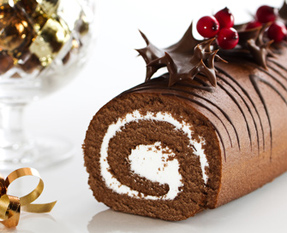
\includegraphics{figure/buche.jpg}
	%	\caption{Exemple typique de bûche risquant de nous retarder.}
	%	\label{fig:buche}
	%\end{figure}

	%On fait la méthode agile pour lécher les boules du prof.

	Nous avons commencé par lister les tâches que nous allons devoir réaliser pour que notre projet soit mené à son terme. Nous les avons ensuite regroupées selon la version pour laquelle elles seront effectuées, puis divisées en sprints. Ceux-ci sont caractéristiques de la méthode Scrum, méthode agile à laquelle nous avons emprunté les concepts de sprint et de réunion de concertation sur l'avancement (même si elles ne sont qu'hebdomadaires). Nous avons ensuite envisagé les différents obstacles qui pourraient nous retarder et avons ensuite pu estimer une durée nécessaire à chaque tâche en tenant compte de ces risques. Notre planification est le résultat de ces estimations. Elle sera soumise à des changements, mais ceci fait partie intégrante des méthodes agiles. Nous pouvons maintenant commencer la conception de \glasir{}, qui détaillera son architecture et son interface graphique.
	\paragraph{Critiques}